\documentclass[tikz,10pt,fleqn]{article}
\usepackage{amsmath}
\usepackage{algorithm}
\usepackage{algpseudocode}
\usepackage{graphicx}
\usepackage{booktabs}
\usepackage{minted}
\usepackage{hyperref}
\usepackage[dvipsnames]{xcolor}
\definecolor{LightGray}{gray}{0.95}
\setminted{
    frame=lines,
    framesep=2mm,
    baselinestretch=1.2,
    bgcolor=LightGray,
    fontsize=\fontsize{8.5}{8.5}\selectfont,
    linenos,
    mathescape=true,
    escapeinside=||,
}


\title{\textbf{Software Analytics\\Bug Triaging}}

\author{Joy Albertini, Jacob Salvi,Adam Kasperski,Anuj Kumar}
\date{}



\begin{document}
\maketitle

\section*{Introduction}
In this report we explain how the solution for the assignment was developed and we highlight some interesting visualizations and analysis of our results.\\
Link to github: \href{https://github.com/JacobSalvi/software-analytics-bug-triaging}{bug triaging}\\
Link to pre-trained models: \href{https://usi365-my.sharepoint.com/:u:/g/personal/alberj_usi_ch/ETIADAeiFuZMpq4sqEEyNdMBL69uAv7qzqJbgXMEkZxUDw?e=zUUBDH}{models}

\section*{Data collection}
\subsection*{Issues collections}
Initially we tried to collect the issues using the 'pygithub' library.\\
We set up the 'github' object, \mintinline{python}{Github(auth=auth, per_page=100)}, to fetch 100 issues per page and then tried to get the issues by iterating over the 'PaginatedList' returned by the \mintinline{python}{repo.get_issues(state="closed")}.\\
This method revealed to be quite slow since a much larger number of requests than expected were performed. With 220000 issue and 100 issues per page a mere 2200 requests should have sufficed, avoiding the 5000 request per hour limit github has in place.\\
Instead a much larger number of requests were performed and we became subject to the timeout put in place by github. \\
To solve this problems we have completely ditched the 'pygithub' library, opting to make the request manually.

\begin{minted}{python}
base_url = "https://api.github.com/repos/microsoft/vscode"
url = f"{base_url}/issues?state=closed&page={current_page}&per_page=100&\
direction=asc"
response = requests.request("GET", url, headers=headers, data=payload)
\end{minted}

By fetching the issues in ascending order we should get issues with issues number increasing from number 1 onward. We limited our search to issues in the closed state, as can be seen from the previous code snippet, and we only kept the issues with exactly one assignee, as shown in the following snippet.\\
\begin{minted}{python}
issues_to_keep = [issue for issue in issues if issue["number"]
<= max_issue_number and len(issue["assignees"]) == 1]
\end{minted}

That said, it seems that the github api itself has a small bug. Page 1921 had an out of place issue.\newpage This page contained issues numbered as [205001, 205002, 205003, 230000, 205004, ...], the obvious outlier was causing issues by triggering an early termination.\\
We saved all of the issues data as received in a json file to be used for the preprocessing. Having all the raw data allowed us to study which part of the data was useful without having to fetch it again.\\

\subsection*{Commits collections}
We extracted commits from the \textbf{main branch} using the GitHub API. Attempting to extract commits from \textbf{all branches} proved challenging due to the high number of commits and GitHub API rate limits. To overcome this, we utilized the \texttt{git log} command to retrieve all commits locally. However, mapping these commits to usernames was difficult because many commits lacked author names and email addresses. We considered fetching usernames by commit SHA through the API, but the rate limits again restricted this method. Consequently, extracting commits from all branches was limited by API constraints and incomplete author information.



\section*{Pre processing}

The data had to be pre-processed before being given to the model for training.
Of all the information we retrieved in the previous step, we decided to keep only the 'title', 'body', 'id', 'number', 'url', 'assignee', and the 'labels'.\\
The title and body required the most preprocessing, given that they contain the bulk of the text.  \\
From the raw data we obtained, we first removed the issue pertaining to pull requests.\\
Then, given that the bodies of the issues are written in Markdown, we have used a Markdown library to parse them.\\
Some elements, such as HTML tags, links, and images have been removed during the parsing. The code blocks are kept exactly as is.\\
The main parts that have been modified then are headings, paragraphs, and lists.

All text was converted to lowercase, and contractions were expanded to standardize word forms. Emojis and special characters were removed to decrease noise in the data, and any residual URLs and email addresses were eliminated. Mentions and hashtags were removed as well. We also normalized whitespace by collapsing multiple spaces into a single space, and we removed the diacritics.
The text was then tokenized, punctuation was removed from tokens, with the exception of keeping the octothorpe in the word 'C\#' and 'F\#', since these are programming language names, and module names. Tokens longer than 40 characters were excluded. We removed common English stopwords and lemmatized the remaining words to their base forms.\\
We used lemmatization as we thought that reducing the word to its base form instead of stemming it would preserve more semantic meaning and yield better results in subsequent steps.


\section*{Predictor} We built our predictor using the base \textbf{RoBERTa} model initially, and the \textbf{RobertaForSequenceClassification} afterwards, which has up to 125 million parameters. With 128 thousand documents and 78 different labels, RoBERTa was more than capable of handling our needs with plenty of room to spare.

\subsection*{Predictor Variables and Corpus} During the development of our model, we experimented with various predictor variables to determine the most effective ones for predicting assignees. Initially, we included seven columns during preprocessing but soon narrowed it down to four key features: \texttt{title}, \texttt{body}, \texttt{labels}, and \texttt{assignee}.

The \texttt{title} and \texttt{body} were essential as they contain the core information about each issue, providing the necessary context for the model to understand the problem.

After several iterations of refinement  of our preprocessing steps, we decided to incorporate issue \textbf{labels} into the training corpus. We believed that users are likely to work on similar issues and thus be assigned tasks with corresponding labels. Nonetheless, the absence of labels in newer issues presented a challenge for maintaining consistent prediction performance.

\subsection*{Embedding} Our Predictor uses a \texttt{LabelEncoder} to convert assignee IDs into numerical labels, facilitating their use in classification tasks and allowing for easy retrieval of user information in the following steps. \\
The core of our model is the RoBERTa-based sequence classification setup, which we configured with the appropriate number of output labels based on our unique assignees.\\
 RoBERTa's strong language understanding helps the model identify patterns and relationships in the text, enabling it to predict assignees accurately.

\subsection*{Training} Training the model involves running through the dataset multiple times, known as epochs. In each epoch, the model processes batches of data, makes predictions, and calculates loss values. These loss values are then used to adjust the model's weights through backpropagation—a crucial step for learning. We use the \texttt{AdamW} optimizer to fine-tune the model's weights, ensuring that the model gradually minimizes the loss and improves its performance over time.

\subsection*{Evaluation} The evaluation method assesses how well the model performs on a test dataset by calculating key metrics such as accuracy, precision, recall, and F1-score. We use tools like classification reports and confusion matrices to gain a detailed understanding of the model's strengths and areas for improvement.

\subsection*{Iterations} In our initial attempt, we used logistic regression for bug classification and achieved only about 30\% accuracy. We realized that logistic regression struggles with the high-dimensional embeddings provided by RoBERTa and doesn't handle overlapping boundaries well—such as when multiple assignees are solving similar bugs—leading to incorrect classifications. These issues limited our ability to improve accuracy. Finally, we switched to using \texttt{RobertaForSequenceClassification} as our base model. This proved to be a much better choice, overcoming the limitations of logistic regression and significantly boosting the model's accuracy.

\section*{Results}
\subsection*{All issues}
With all issues included in the training corpus the model took multiple hours to train and we achieved an accuracy of roughly \textbf{61\%}.\\
In the following table we can observe some statistics about the performance of the model per each assignee.\\
The precision is simply given by the ratio between correct predictions and total predictions, while the recall measures how many issues that should have been assigned to a given assignee were actually assigned to him.\\
There seems to be a correlation between the number of predictions and the precision and between the recall and the number of predictions.\\
We used a simple python script to calculate this correlation:
\begin{minted}{python}
	....
    df = pd.DataFrame(data)
    tau, p_value = kendalltau(df['Total Predictions'], df['Precision'])
    print(f"Correlation coefficient: {tau}")
\end{minted}

And we get a correlation coefficient of $0.45\sim$ for the precision and $0.67\sim$ for the recall, meaning that there is a weak correlation between precision and number of predictions and a moderate correlation between the recall and the number of predictions.\\
This result is slightly surprising since we expected a sharper correlation between the computed statistics and the number of predictions.


\begin{table}[H]
    \centering
    \caption{Assignee performance for all issues.}
    \begin{tabular}{@{}lcccccc@{}}
        \toprule
        Assignee & Precision & Recall & Total Predictions & Correct Predictions \\ \midrule
        lszomoru       & 0.894  & 0.664  & 104 & 93  \\
        mjbvz          & 0.804  & 0.862  & 419 & 337 \\
        meganrogge     & 0.790  & 0.716  & 252 & 199 \\
        sandy081       & 0.766  & 0.810  & 184 & 141 \\
        rzhao271       & 0.760  & 0.514  & 25  & 19  \\
        andreamah      & 0.729  & 0.507  & 48  & 35  \\
        Yoyokrazy      & 0.714  & 0.286  & 14  & 10  \\
        benibenj       & 0.704  & 0.241  & 27  & 19  \\
        lramos15       & 0.703  & 0.683  & 101 & 71  \\
        hediet         & 0.692  & 0.365  & 39  & 27  \\
        roblourens     & 0.688  & 0.661  & 298 & 205 \\
        Tyriar         & 0.615  & 0.770  & 169 & 104 \\
        jrieken        & 0.585  & 0.703  & 142 & 83  \\
        aiday-mar      & 0.571  & 0.327  & 28  & 16  \\
        aeschli        & 0.567  & 0.529  & 97  & 55  \\
        connor4312     & 0.548  & 0.479  & 84  & 46  \\
        alexr00        & 0.450  & 0.545  & 80  & 36  \\
        justschen      & 0.444  & 0.302  & 36  & 16  \\
        alexdima       & 0.436  & 0.459  & 39  & 17  \\
        TylerLeonhardt & 0.430  & 0.623  & 100 & 43  \\
        deepak1556     & 0.417  & 0.495  & 120 & 50  \\
        rebornix       & 0.412  & 0.519  & 34  & 14  \\
        bpasero        & 0.342  & 0.534  & 184 & 63  \\
        amunger        & 0.333  & 0.429  & 18  & 6   \\
        chrmarti       & 0.259  & 0.259  & 27  & 7   \\
        joaomoreno     & 0.255  & 0.394  & 51  & 13  \\
        sbatten        & 0.241  & 0.875  & 29  & 7   \\
        daviddossett   & 0.200  & 0.071  & 5   & 1   \\
        ulugbekna      & 0.176  & 0.261  & 34  & 6   \\
        bhavyaus       & 0.056  & 0.167  & 72  & 4   \\
        isidorn        & 0.000  & 0.000  & 4   & 0   \\
        dbaeumer       & 0.000  & 0.000  & 2   & 0   \\
        DonJayamanne   & 0.000  & 0.000  & 1   & 0   \\
        karthiknadig   & 0.000  & 0.000  & 0   & 0   \\
        joyceerhl      & 0.000  & 0.000  & 8   & 0   \\ \bottomrule
    \end{tabular}
\end{table}

\subsection*{Recent issues}
Limiting our training to recent issues, the model was significantly faster to train and we achieved an accuracy of roughly \textbf{ 57\%}.\\
This results was slightly puzzling given that we expected the model to do better on only recent issues since these should be more relevant.\\
We assume that the sheer amount of information obtained using all of the issues offset any advantage that limiting the training to recent issues might give.\\
The correlation between precision and number of prediction is slightly better at 0.48, but it is still weak.\\
The correlation between recall and predictions is 0.77 which give quite a strong correlation.

\begin{table}[H]
    \centering
    \caption{Assignee performance for recent issues.}
    \begin{tabular}{@{}lcccccc@{}}
        \toprule
        Assignee & Precision & Recall & Total Predictions & Correct Predictions \\ \midrule
        lszomoru       & 0.782 & 0.743  & 133 & 104 \\
        mjbvz          & 0.768 & 0.752  & 383 & 294 \\
        sandy081       & 0.728 & 0.770  & 184 & 134 \\
        Tyriar         & 0.713 & 0.533  & 101 & 72  \\
        roblourens     & 0.691 & 0.648  & 291 & 201 \\
        amunger        & 0.667 & 0.143  & 3   & 2   \\
        meganrogge     & 0.667 & 0.856  & 357 & 238 \\
        benibenj       & 0.667 & 0.228  & 27  & 18  \\
        andreamah      & 0.644 & 0.551  & 59  & 38  \\
        aiday-mar      & 0.636 & 0.286  & 22  & 14  \\
        lramos15       & 0.575 & 0.663  & 120 & 69  \\
        TylerLeonhardt & 0.571 & 0.464  & 56  & 32  \\
        jrieken        & 0.548 & 0.585  & 126 & 69  \\
        Yoyokrazy      & 0.533 & 0.229  & 15  & 8   \\
        alexr00        & 0.510 & 0.394  & 51  & 26  \\
        justschen      & 0.500 & 0.302  & 32  & 16  \\
        connor4312     & 0.488 & 0.438  & 86  & 42  \\
        aeschli        & 0.454 & 0.471  & 108 & 49  \\
        rzhao271       & 0.436 & 0.459  & 39  & 17  \\
        rebornix       & 0.421 & 0.889  & 57  & 24  \\
        bpasero        & 0.359 & 0.475  & 156 & 56  \\
        joaomoreno     & 0.325 & 0.394  & 40  & 13  \\
        deepak1556     & 0.301 & 0.574  & 193 & 58  \\
        alexdima       & 0.298 & 0.459  & 57  & 17  \\
        chrmarti       & 0.273 & 0.111  & 11  & 3   \\
        ulugbekna      & 0.235 & 0.174  & 17  & 4   \\
        hediet         & 0.222 & 0.405  & 135 & 30  \\
        sbatten        & 0.174 & 0.500  & 23  & 4   \\
        isidorn        & 0.000 & 0.000  & 0   & 0   \\
        dbaeumer       & 0.000 & 0.000  & 0   & 0   \\
        DonJayamanne   & 0.000 & 0.000  & 0   & 0   \\
        karthiknadig   & 0.000 & 0.000  & 0   & 0   \\
        bhavyaus       & 0.000 & 0.000  & 1   & 0   \\
        daviddossett   & 0.000 & 0.000  & 0   & 0   \\
        joyceerhl      & 0.000 & 0.000  & 0   & 0   \\ \bottomrule
    \end{tabular}
\end{table}

\subsection*{Clusters}
\subsubsection{Train set issues cluster}
We thought it could have been interesting to see how the issues and assignee are clustered.\\
From the following image can be observed that the issues form quite well defined and disjointed clusters around their assigned Assignee.\\
It would thus be natural to attempt to classify new documents based on these clusters to assign them to a user.\\
This information can be used to validate our results and potentially even to refine the model further.
The image below represent a sample of the train set.
\begin{table}[H]
	\centering
	\caption{Clustering of issues in relation to assignees}
	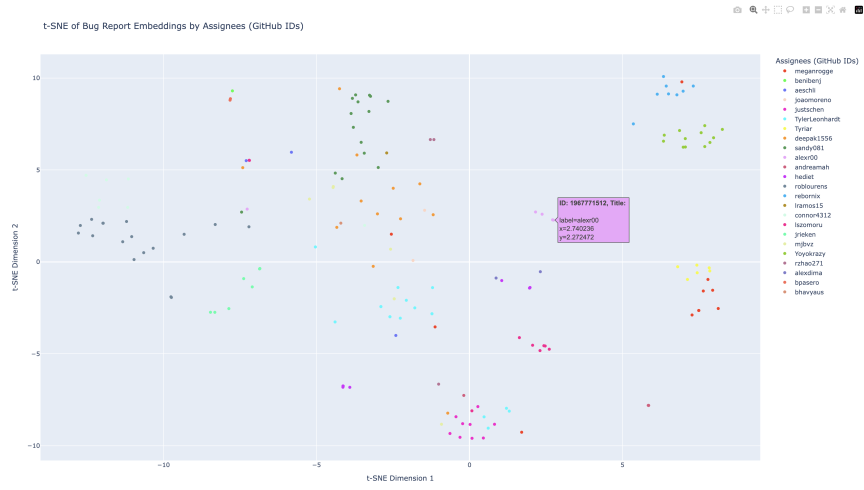
\includegraphics[width=\textwidth]{plot.png}
\end{table}
\subsubsection{Recent issues cluster}
The image below illustrates a sample of the training set. It is evident that the clusters are less well-defined in this instance. This ambiguity could contribute to the lower accuracy observed with recent issues. Additionally, there may be increased variability between assignees and issue documents.
\begin{table}[H]
	\centering
	\caption{Clustering of issues in relation to assignees}
	\includegraphics[width=\textwidth]{plot2.png}
\end{table}


\begin{table}[H]
	\centering
	\caption{Clustering of issues in relation to assignees}
	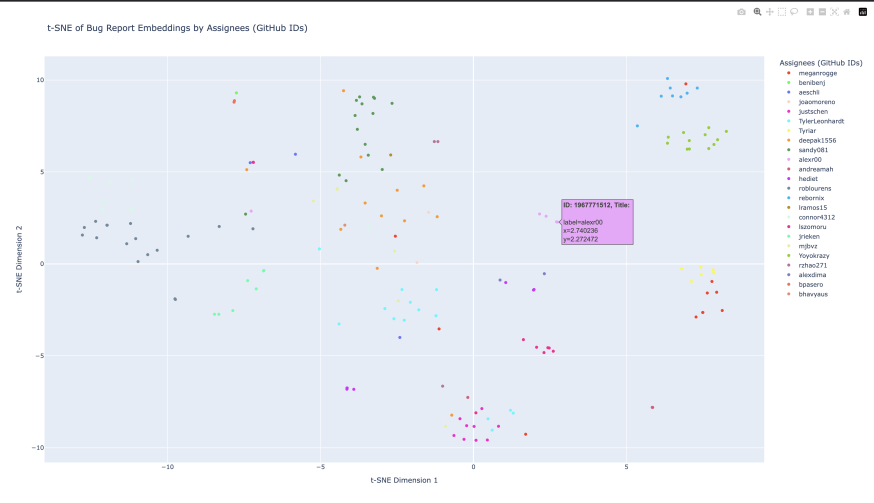
\includegraphics[width=\textwidth]{plot_sparse.png}
\end{table}
\section*{Interface}
We included a simple terminal-based interface to query the top five most likely assignee given an issue number.\\
We opted for this kind of interface instead of a web based approach since this can easily be run on the server but still allows for a degree of interaction.
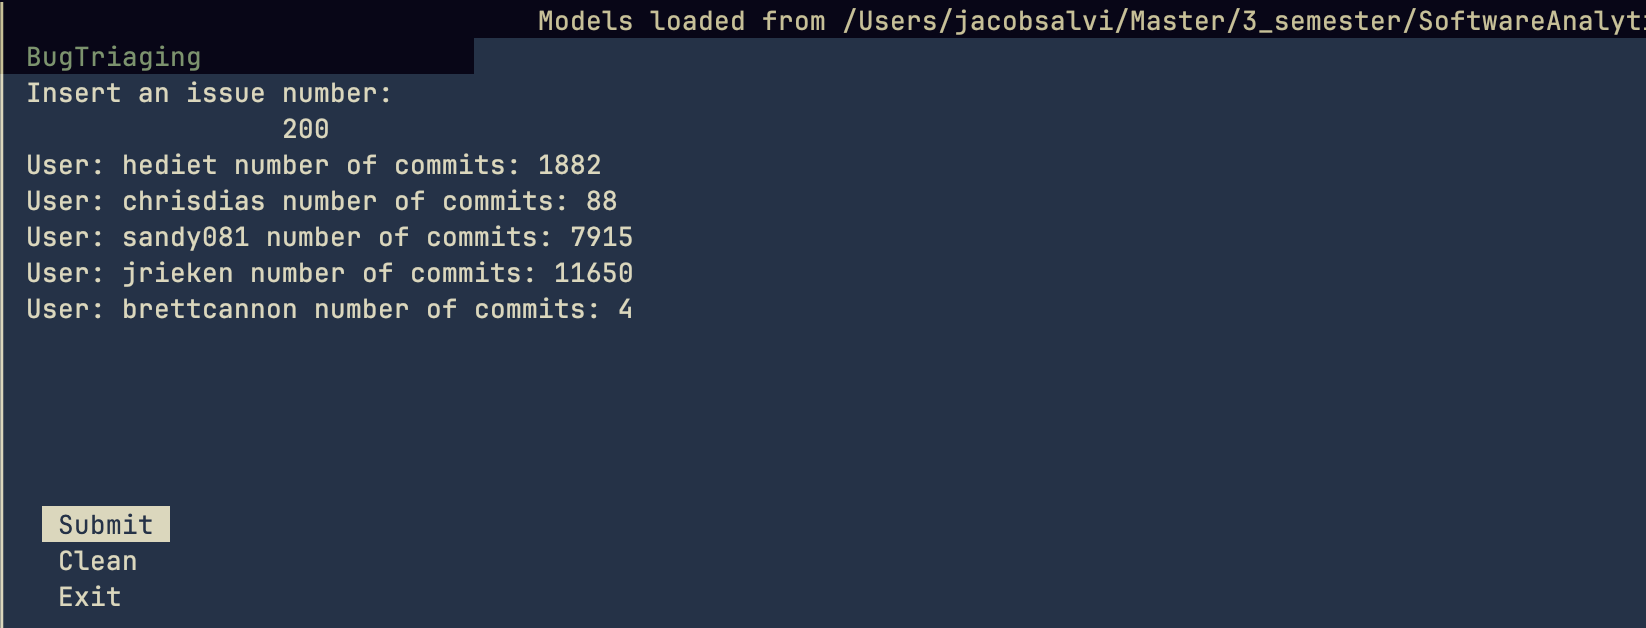
\includegraphics[width=\textwidth]{./tui.png}

To run it is sufficient to run the following code, given that the python environment is set up as described in the README.
\begin{minted}{bash}
python3 src/tui/tui.py
\end{minted}

\section*{Conclusion}
In the project we had the chance of developing a tool for automated bug triaging leveraging machine learning.\\
Developing this tool we came to appreciate both the strength of such an approach to solve this kind of problems and the challenges faced in developing it.\\
We also appreciated doing this kind of work in a quite realistic context, given that the vscode repository was used, and can picture many practical applications of similar techniques to solve similar challenges in industry.\\
It is also our opinion that we achieved satisfactory results in terms of accuracy.

\end{document}
